本アプリの依頼側、配達側、店舗側そして管理側の各機能設計について記述する。
\subsection{機能概要図}
以下に示す図は本アプリの機能概要である。

\subsubsection{依頼側}
\begin{figure}[H]
  \centering
  \includegraphics[width=0.75\textwidth]{./Image/画面遷移図/依頼側遷移図.pdf}
  \caption{依頼側機能概要図}
  \label{fig:依頼側機能概要図}
\end{figure}


\subsubsection{配達側}
\begin{figure}[H]
  \centering
  \includegraphics[width=0.75\textwidth]{./Image/画面遷移図/配達側遷移図.pdf}
  \caption{配達側機能概要図}
  \label{fig:配達側機能概要図}
\end{figure}


\subsubsection{店舗側}
\begin{figure}[H]
  \centering
  \includegraphics[width=0.75\textwidth]{./drawio遷移図/店舗画面遷移図改.drawio.pdf}
  \caption{店舗側機能概要図}
  \label{fig:店舗側機能概要図}
\end{figure}

\subsubsection{管理者側}
\begin{figure}[H]
  \centering
  \includegraphics[width=0.75\textwidth]{./Image/画面遷移図/管理者側遷移図_修正版.pdf}
  \caption{管理者側機能概要図}
  \label{fig:管理者側機能概要図}
\end{figure}



\subsubsection{ログイン関連機能}
図\ref{fig:ログイン関連機能}は、ログイン関連機能の概要図である。
\begin{figure}[H]
  \centering
  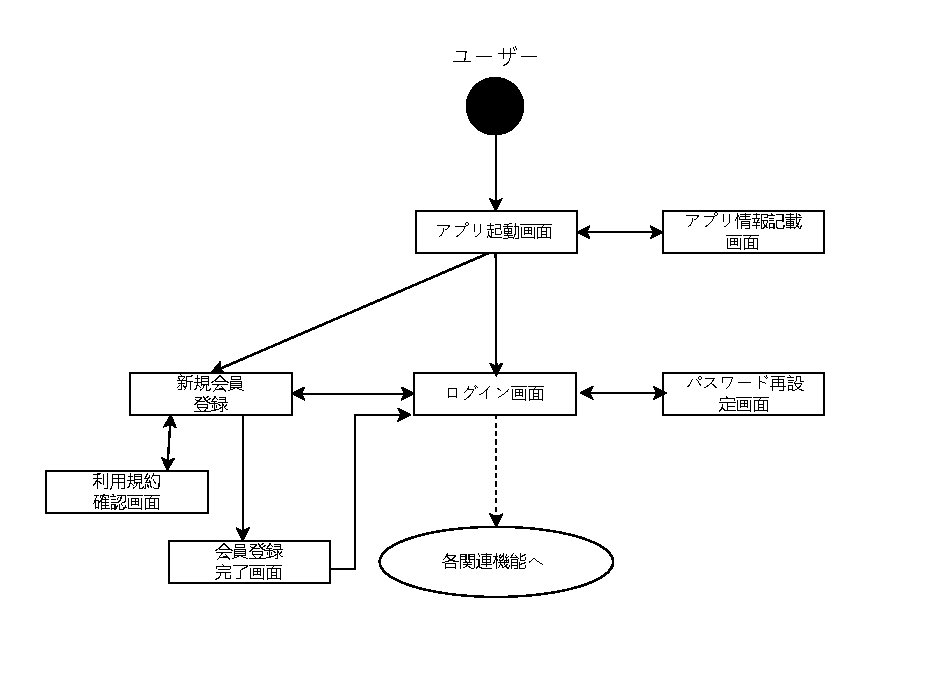
\includegraphics[width=0.75\textwidth]{./Image/ログイン関連機能.pdf}
  \caption{ログイン関連機能}
  \label{fig:ログイン関連機能}
\end{figure}



\subsection{共通機能}
本アプリの依頼側、配達側、店舗側そして管理側の共通の機能設計を以下に記述する。
\subsubsection{新規会員登録機能}
依頼側と配達側、店舗側が利用規約に同意し、情報を入力し、その情報に不備がなく、送信されたメールで本人確認を行うこ
とで、新規会員登録ができる機能である。また、入力情報として、配達側と依頼側は名前、性別、生年月日、住所、メールアドレス
、電話番号、パスワード、パスワード(確認)を、店舗側は店舗所在地、飲食店営業許可書のファイルおよび写真、メールア
ドレスまたは電話番号、パスワード、パスワード(確認)を入力する。

\begin{figure}[H]
  \centering
  \includegraphics[width=0.75\textwidth]{./Image/新規会員登録機能.pdf}
  \caption{新規会員登録機能}
  \label{fig:新規会員登録機能}
\end{figure}

\subsubsection{マイページ}
会員の情報を取得し、そのユーザが会員情報の確認・変更や、ログアウト、退会などが行える画面を表示させる機能で
ある。

\begin{figure}[H]
  \centering
  \includegraphics[width=0.75\textwidth]{./Image/マイページ機能.pdf}
  \caption{マイページ機能}
  \label{fig:マイページ機能}
\end{figure}
\clearpage

\subsubsection{ログイン}
アプリ起動時に会員登録済みの利用者(依頼側、配達側、店舗側そして管理側)が、自身のログイン情報を入力することで、
アプリのサービスを利用できるようにする機能である。依頼側、配達側、店舗側はメールアドレスとパスワードを、管理側は
管理者IDとパスワードを入力して、ログインする。

\begin{figure}[H]
  \centering
  \includegraphics[width=0.75\textwidth]{./Image/ログイン.pdf}
  \caption{ログイン機能}
  \label{fig:ログイン}
\end{figure}
\clearpage

\subsubsection{ログアウト}
ログアウトを選択することで、ログイン前の状態に戻す機能で、ログイン画面に遷移する。

\begin{figure}[H]
  \centering
  \includegraphics[width=0.75\textwidth]{./Image/ログアウト.pdf}
  \caption{ログアウト機能}
  \label{fig:ログアウト}
\end{figure}
\clearpage

\subsubsection{退会}
会員が任意のタイミングでアプリ会員から退会する機能。会員情報をデータベースから完全に削除する。

\begin{figure}[H]
  \centering
  \includegraphics[width=0.75\textwidth]{./Image/退会.pdf}
  \caption{退会機能}
  \label{fig:退会}
\end{figure}
\clearpage

\subsubsection{パスワード再発行}
ユーザーはパスワードを忘れた場合、メールアドレスをフォームに入力することで再発行を行う。間違っている場
合はエラーメッセージを出力し、合っている場合はパスワードを生成してデータベースを更新し、メールアドレス宛にそのパス
ワードを送信し、通知画面を表示する。

\begin{figure}[H]
  \centering
  \includegraphics[width=0.75\textwidth]{./Image/パスワード再発行.pdf}
  \caption{パスワード再発行機能}
  \label{fig:パスワード再発行}
\end{figure}
\clearpage

\subsubsection{会員情報確認・変更}
会員がアプリ内のホームページ画面から自身の会員情報を確認・変更するための機能である。

\begin{figure}[H]
  \centering
  \includegraphics[width=0.75\textwidth]{./Image/会員情報確認変更.pdf}
  \caption{会員情報確認・変更}
  \label{fig:会員情報確認変更}
\end{figure}
\clearpage

\subsubsection{問い合わせ}
会員がアプリの操作方法などの問い合わせを管理者に対して行うための機能である。
問い合わせへの回答は会員登録したメールアドレスに送信される。

\begin{figure}[H]
  \centering
  \includegraphics[width=0.75\textwidth]{./Image/問い合わせ機能.pdf}
  \caption{問い合わせ機能}
  \label{fig:問い合わせ機能}
\end{figure}
\clearpage

\subsection{依頼側}
\subsubsection{商品一覧}
図\ref{fig:依頼者側商品一覧}は、依頼者が注文可能な商品の一覧を表示する機能である。
\begin{figure}[H]
  \centering
  \includegraphics[width=0.75\textwidth]{./Image/依頼者側商品一覧.pdf}
  \caption{商品一覧機能}
  \label{fig:依頼者側商品一覧}
\end{figure}
\clearpage

\subsubsection{注文}
図\ref{fig:依頼者側注文}は、商品を選択し、注文を行う機能である。
\begin{figure}[H]
  \centering
  \includegraphics[width=0.75\textwidth]{./Image/依頼者側注文画面.pdf}
  \caption{注文機能}
  \label{fig:依頼者側注文}
\end{figure}
\clearpage

\subsubsection{カート}
図\ref{fig:依頼者側カート}は、注文予定の商品を確認・編集するカート機能である。
\begin{figure}[H]
  \centering
  \includegraphics[width=0.75\textwidth]{./Image/依頼者側カート画面.pdf}
  \caption{カート機能}
  \label{fig:依頼者側カート}
\end{figure}
\clearpage

\subsubsection{購入承認}
図\ref{fig:依頼者側購入承認}は、注文内容を確認し、購入を確定する機能である。
\begin{figure}[H]
  \centering
  \includegraphics[width=0.75\textwidth]{./Image/依頼者側購入承認.pdf}
  \caption{購入承認機能}
  \label{fig:依頼者側購入承認}
\end{figure}
\clearpage

\subsubsection{支払い明細表示}
図\ref{fig:依頼者側支払い明細表示}は、支払いの明細を表示する機能である。
\begin{figure}[H]
  \centering
  \includegraphics[width=0.75\textwidth]{./Image/依頼者側支払い明細表示.pdf}
  \caption{支払い明細表示機能}
  \label{fig:依頼者側支払い明細表示}
\end{figure}
\clearpage

\subsubsection{マップ}
図\ref{fig:依頼者側マップ}は、店舗や配達員の位置などをマップ上で確認する機能である。
\begin{figure}[H]
  \centering
  \includegraphics[width=0.75\textwidth]{./Image/依頼者側マップ画面.pdf}
  \caption{マップ機能}
  \label{fig:依頼者側マップ}
\end{figure}
\clearpage

\subsubsection{商品到着報告}
図\ref{fig:依頼者側商品到着報告}は、商品が到着したことを報告する機能である。
\begin{figure}[H]
  \centering
  \includegraphics[width=0.75\textwidth]{./Image/依頼者側商品到着報告画面.pdf}
  \caption{商品到着報告機能}
  \label{fig:依頼者側商品到着報告}
\end{figure}
\clearpage

\subsubsection{店舗評価}
図\ref{fig:依頼者側店舗評価}は、利用した店舗を評価する機能である。
\begin{figure}[H]
  \centering
  \includegraphics[width=0.75\textwidth]{./Image/依頼者側店舗評価.pdf}
  \caption{店舗評価機能}
  \label{fig:依頼者側店舗評価}
\end{figure}
\clearpage

\subsubsection{配達員評価}
図\ref{fig:依頼者側配達員評価}は、担当した配達員を評価する機能である。
\begin{figure}[H]
  \centering
  \includegraphics[width=0.75\textwidth]{./Image/依頼者側配達員評価.pdf}
  \caption{配達員評価機能}
  \label{fig:依頼者側配達員評価}
\end{figure}
\clearpage

\subsubsection{注文履歴一覧}
図\ref{fig:依頼者側注文履歴一覧}は、過去の注文履歴を一覧表示する機能である。
\begin{figure}[H]
  \centering
  \includegraphics[width=0.75\textwidth]{./Image/依頼者側注文履歴一覧画面.pdf}
  \caption{注文履歴一覧機能}
  \label{fig:依頼者側注文履歴一覧}
\end{figure}
\clearpage

\subsubsection{注文履歴詳細}
図\ref{fig:依頼者側注文履歴詳細}は、注文履歴の詳細を確認する機能である。
\begin{figure}[H]
  \centering
  \includegraphics[width=0.75\textwidth]{./Image/依頼者側注文履歴詳細画面.pdf}
  \caption{注文履歴詳細機能}
  \label{fig:依頼者側注文履歴詳細}
\end{figure}
\clearpage

\subsubsection{配達先住所確認・編集}
図\ref{fig:依頼者側配達先住所確認・編集}は、配達先の住所を確認・編集する機能である。
\begin{figure}[H]
  \centering
  \includegraphics[width=0.75\textwidth]{./Image/依頼者側配達先住所確認・編集画面.pdf}
  \caption{配達先住所確認・編集機能}
  \label{fig:依頼者側配達先住所確認・編集}
\end{figure}
\clearpage

\subsubsection{口座情報登録・確認}
図\ref{fig:依頼者側口座情報登録・確認}は、支払い等に使用する口座情報を登録・確認する機能である。
\begin{figure}[H]
  \centering
  \includegraphics[width=0.75\textwidth]{./Image/依頼者側口座情報登録・確認画面.pdf}
  \caption{口座情報登録・確認機能}
  \label{fig:依頼者側口座情報登録・確認}
\end{figure}
\clearpage

\subsubsection{通知}
図\ref{fig:依頼者側通知}は、依頼者宛の通知を表示する機能である。
\begin{figure}[H]
  \centering
  \includegraphics[width=0.75\textwidth]{./Image/依頼者側通知画面.pdf}
  \caption{通知機能}
  \label{fig:依頼者側通知}
\end{figure}
\clearpage

\subsubsection{マイページ}
図\ref{fig:依頼者側マイページ}は、依頼者のマイページを表示する機能である。
\begin{figure}[H]
  \centering
  \includegraphics[width=0.75\textwidth]{./Image/依頼者側マイページ画面.pdf}
  \caption{マイページ機能}
  \label{fig:依頼者側マイページ}
\end{figure}
\clearpage

\subsubsection{会員情報確認・編集}
図\ref{fig:依頼者側会員情報確認・編集}は、会員情報の確認および編集を行う機能である。
\begin{figure}[H]
  \centering
  \includegraphics[width=0.75\textwidth]{./Image/依頼者側会員情報確認・編集画面.pdf}
  \caption{会員情報確認・編集機能}
  \label{fig:依頼者側会員情報確認・編集}
\end{figure}
\clearpage

\subsubsection{パスワード変更}
図\ref{fig:依頼者側パスワード変更}は、パスワードを変更する機能である。
\begin{figure}[H]
  \centering
  \includegraphics[width=0.75\textwidth]{./Image/依頼者側パスワード変更.pdf}
  \caption{パスワード変更機能}
  \label{fig:依頼者側パスワード変更}
\end{figure}
\clearpage

\subsubsection{ログアウト}
図\ref{fig:依頼者側ログアウト}は、ログアウトを行う機能である。
\begin{figure}[H]
  \centering
  \includegraphics[width=0.75\textwidth]{./Image/依頼者側ログアウト画面.pdf}
  \caption{ログアウト機能}
  \label{fig:依頼者側ログアウト}
\end{figure}
\clearpage

\subsubsection{退会}
図\ref{fig:依頼者側退会}は、退会手続きを行う機能である。
\begin{figure}[H]
  \centering
  \includegraphics[width=0.75\textwidth]{./Image/依頼者側退会画面.pdf}
  \caption{退会機能}
  \label{fig:依頼者側退会}
\end{figure}
\clearpage

\subsubsection{問い合わせ}
図\ref{fig:依頼者側問い合わせ}は、運営への問い合わせを行う機能である。
\begin{figure}[H]
  \centering
  \includegraphics[width=0.75\textwidth]{./Image/依頼者側問い合わせ.pdf}
  \caption{問い合わせ機能}
  \label{fig:依頼者側問い合わせ}
\end{figure}
\clearpage

\subsection{配達側}
\subsubsection{口座情報変更}
配達員が任意のタイミングで口座情報を変更する機能である。
\begin{figure}[H]
  \centering
  \includegraphics[width=0.75\textwidth]{./Image/deliverer機能設計/口座情報変更機能.pdf}
  \caption{口座情報変更機能}
  \label{fig:口座情報変更機能}
\end{figure}
\clearpage

\subsubsection{履歴書記述}
求人応募の際に必要となる履歴書情報を記述する機能である。
\begin{figure}[H]
  \centering
  \includegraphics[width=0.75\textwidth]{./Image/deliverer機能設計/履歴書記述機能.pdf}
  \caption{履歴書記述機能}
  \label{fig:履歴書記述機能}
\end{figure}
\clearpage

\subsubsection{マップ}
マップと配達ルートを表示する機能である。
\begin{figure}[H]
  \centering
  \includegraphics[width=0.75\textwidth]{./Image/deliverer機能設計/マップ.pdf}
  \caption{マップ機能}
  \label{fig:マップ}
\end{figure}
\clearpage

\subsubsection{求人検索}
求人検索する機能である。
\begin{figure}[H]
  \centering
  \includegraphics[width=0.75\textwidth]{./Image/deliverer機能設計/求人検索機能.pdf}
  \caption{求人検索機能}
  \label{fig:求人検索機能}
\end{figure}
\clearpage

\subsubsection{給与明細}
給与明細を表示する機能である。
\begin{figure}[H]
  \centering
  \includegraphics[width=0.75\textwidth]{./Image/deliverer機能設計/給与明細機能.pdf}
  \caption{給与明細表示機能}
  \label{fig:給与明細機能}
\end{figure}
\clearpage

\subsubsection{配達履歴}
配達履歴を表示する機能である。
\begin{figure}[H]
  \centering
  \includegraphics[width=0.75\textwidth]{./Image/deliverer機能設計/配達履歴.pdf}
  \caption{配達履歴表示機能}
  \label{fig:配達履歴}
\end{figure}
\clearpage

\subsubsection{配達員用通知}
配達用の通知を表示する機能である。
\begin{figure}[H]
  \centering
  \includegraphics[width=0.75\textwidth]{./Image/deliverer機能設計/deliverer通知機能.pdf}
  \caption{配達員用通知機能}
  \label{fig:deliverer通知機能}
\end{figure}

\subsubsection{パスワード変更前のパスワード認証}
パスワード変更を行うにあたり、現在のパスワード認証を行う機能である。
\begin{figure}[H]
  \centering
  \includegraphics[width=0.75\textwidth]{./Image/deliverer機能設計/マイページ_パスワード認証.pdf}
  \caption{パスワード変更における現在のパスワード認証機能}
  \label{fig:パスワード認証}
\end{figure}

\subsubsection{パスワード変更}
パスワード変更および更新を行う機能である。
\begin{figure}[H]
  \centering
  \includegraphics[width=0.75\textwidth]{./Image/deliverer機能設計/マイページ_パスワード変更.pdf}
  \caption{パスワード変更および更新機能}
  \label{fig:パスワード変更および更新}
\end{figure}

\clearpage

\subsection{店舗側}

\subsubsection{在庫ステータス変更機能}
商品の在庫の状況を変更する機能である。
\begin{figure}[H]
  \centering
  \includegraphics[width=0.75\textwidth]{./Image/店舗在庫ステータス変更機能.drawio.pdf}
  \caption{在庫ステータス変更機能}
  \label{fig:在庫ステータス変更機能}
\end{figure}
\clearpage


\subsubsection{メニュー登録機能}
店舗のメニューを登録する機能である。
\begin{figure}[H]
  \centering
  \includegraphics[width=0.75\textwidth]{./Image/店舗側メニュー登録機能改.drawio.pdf}
  \caption{メニュー登録機能}
  \label{fig:メニュー登録機能}
\end{figure}
\clearpage

\subsubsection{メニュー削除機能}
メニューを削除する機能である。
\begin{figure}[H]
  \centering
  \includegraphics[width=0.75\textwidth]{./Image/店舗側メニュー削除機能改.drawio.pdf}
  \caption{メニュー削除機能}
  \label{fig:メニュー削除機能}
\end{figure}
\clearpage

\subsubsection{メニュー情報変更機能}
メニュー情報を変更する機能である。
\begin{figure}[H]
  \centering
  \includegraphics[width=0.75\textwidth]{./Image/店舗側メニュー編集機能改.drawio.pdf}
  \caption{メニュー情報変更機能}
  \label{fig:メニュー情報変更機能}
\end{figure}
\clearpage

\subsubsection{受注一覧}
受注一覧を表示する機能である。
\begin{figure}[H]
  \centering
  \includegraphics[width=0.75\textwidth]{./Image/店舗受注一覧機能.drawio.pdf}
  \caption{受注一覧機能}
  \label{fig:受注一覧機能}
\end{figure}
\clearpage

\subsubsection{配達員情報確認}
配達員の情報を確認する機能である。
\begin{figure}[H]
  \centering
  \includegraphics[width=0.75\textwidth]{./Image/店舗配達員情報確認.drawio.pdf}
  \caption{配達員情報確認機能}
  \label{fig:配達員情報確認機能}
\end{figure}
\clearpage

\subsubsection{受け渡し完了確認機能}
商品の受け渡し完了を確認する機能である。
\begin{figure}[H]
  \centering
  \includegraphics[width=0.75\textwidth]{./Image/店舗側受け渡し確認機能改.drawio.pdf}
  \caption{受け渡し完了確認機能}
  \label{fig:受け渡し完了確認機能}
\end{figure}
\clearpage

\subsubsection{配達トラブル報告機能}
配達に関するトラブルを報告する機能である。
\begin{figure}[H]
  \centering
  \includegraphics[width=0.75\textwidth]{./Image/店舗側配達トラブル報告機能改.drawio.pdf}
  \caption{配達トラブル報告機能}
  \label{fig:配達トラブル報告機能}
\end{figure}
\clearpage


\subsubsection{売上確認機能}
売上に関する情報を確認する機能である。
\begin{figure}[H]
  \centering
  \includegraphics[width=0.75\textwidth]{./Image/店舗売上画面.drawio.pdf}
  \caption{売上確認機能}
  \label{fig:売上確認機能}
\end{figure}
\clearpage

\subsubsection{売り上げ数確認機能}
売り上げ数に関する情報を確認する機能である。
\begin{figure}[H]
  \centering
  \includegraphics[width=0.75\textwidth]{./Image/店舗売り上げ数管理機能.drawio.pdf}
  \caption{売り上げ数確認機能}
  \label{fig:売り上げ数確認機能}
\end{figure}
\clearpage

\subsubsection{明細表示機能}
売り上げや管理者への手数料を表示する機能である。
\begin{figure}[H]
  \centering
  \includegraphics[width=0.75\textwidth]{./Image/店舗明細表示機能.drawio.pdf}
  \caption{明細表示機能}
  \label{fig:明細表示機能}
\end{figure}
\clearpage


\subsection{管理側}
\subsubsection{アカウント情報登録}
アカウント情報を登録する機能である。
\begin{figure}[H]
  \centering
  \includegraphics[width=0.75\textwidth]{./Image/administrator機能設計/アカウント情報登録機能.pdf}
  \caption{アカウント情報登録機能}
  \label{fig:アカウント情報登録機能}
\end{figure}
\clearpage

\subsubsection{アカウント情報削除}
アカウント情報を削除する機能である。
\begin{figure}[H]
  \centering
  \includegraphics[width=0.75\textwidth]{./Image/administrator機能設計/アカウント情報削除機能.pdf}
  \caption{アカウント情報削除機能}
  \label{fig:アカウント情報削除機能}
\end{figure}
\clearpage

\subsubsection{アカウント情報編集}
アカウント情報を編集する機能である。
\begin{figure}[H]
  \centering
  \includegraphics[width=0.75\textwidth]{./Image/administrator機能設計/アカウント情報編集機能.pdf}
  \caption{アカウント情報編集機能}
  \label{fig:アカウント情報編集機能}
\end{figure}
\clearpage

\subsubsection{アカウントID検索}
各種アカウント管理画面(依頼者、配達員、店舗、管理者)でアカウントIDを検索する機能である。
\begin{figure}[H]
  \centering
  \includegraphics[width=0.75\textwidth]{./Image/administrator機能設計/アカウントID検索機能.pdf}
  \caption{アカウントID検索機能}
  \label{fig:アカウントID検索機能}
\end{figure}
\clearpage

\subsubsection{アカウント名検索}
各種アカウント管理画面(依頼者、配達員、店舗、管理者)でアカウントの名前を検索する機能である。
\begin{figure}[H]
  \centering
  \includegraphics[width=0.75\textwidth]{./Image/administrator機能設計/アカウント氏名検索機能.pdf}
  \caption{アカウント名検索機能}
  \label{fig:アカウント名検索機能}
\end{figure}
\clearpage

\subsubsection{申請確認}
配達員や店舗から申請があったときに、申請の確認・承認を行う機能である。
\begin{figure}[H]
  \centering
  \includegraphics[width=0.75\textwidth]{./Image/administrator機能設計/申請確認機能.pdf}
  \caption{申請確認機能}
  \label{fig:申請確認機能}
\end{figure}
\clearpage

\subsubsection{依頼者アカウント管理画面表示}
依頼者アカウント管理画面の表示を行う機能である。
\begin{figure}[H]
  \centering
  \includegraphics[width=0.75\textwidth]{./Image/administrator機能設計/依頼者アカウント管理画面.pdf}
  \caption{依頼者アカウント管理画面表示機能}
  \label{fig:依頼者アカウント管理画面表示機能}
\end{figure}
\clearpage

\subsubsection{依頼者詳細表示}
依頼者アカウントの詳細の表示を行う機能である。
\begin{figure}[H]
  \centering
  \includegraphics[width=0.75\textwidth]{./Image/administrator機能設計/依頼者詳細表示機能.pdf}
  \caption{依頼者詳細表示機能}
  \label{fig:依頼者詳細表示機能}
\end{figure}
\clearpage

\subsubsection{依頼者注文履歴情報表示}
依頼者アカウントの注文履歴の表示を行う機能である。
\begin{figure}[H]
  \centering
  \includegraphics[width=0.75\textwidth]{./Image/administrator機能設計/依頼者注文履歴情報表示機能.pdf}
  \caption{依頼者注文履歴情報表示機能}
  \label{fig:依頼者注文履歴情報表示機能}
\end{figure}
\clearpage


\subsubsection{依頼者アカウント情報詳細表示}
依頼者アカウント情報の詳細の表示を行う機能である。
\begin{figure}[H]
  \centering
  \includegraphics[width=0.75\textwidth]{./Image/administrator機能設計/依頼者アカウント情報詳細表示機能.pdf}
  \caption{依頼者アカウント情報詳細表示機能}
  \label{fig:依頼者アカウント情報詳細表示機能}
\end{figure}
\clearpage

\subsubsection{配達員アカウント管理画面表示}
配達員アカウント管理画面の表示を行う機能である。
\begin{figure}[H]
  \centering
  \includegraphics[width=0.75\textwidth]{./Image/administrator機能設計/配達員アカウント管理画面.pdf}
  \caption{配達員アカウント管理画面表示機能}
  \label{fig:配達員アカウント管理画面表示機能}
\end{figure}
\clearpage

\subsubsection{配達員詳細表示}
配達員アカウントの詳細の表示を行う機能である。
\begin{figure}[H]
  \centering
  \includegraphics[width=0.75\textwidth]{./Image/administrator機能設計/配達員詳細表示機能.pdf}
  \caption{配達員詳細表示機能}
  \label{fig:配達員詳細表示機能}
\end{figure}
\clearpage

\subsubsection{履歴書表示}
配達員詳細画面から履歴書の表示を行う機能である。
\begin{figure}[H]
  \centering
  \includegraphics[width=0.75\textwidth]{./Image/administrator機能設計/履歴書表示機能.pdf}
  \caption{履歴書表示機能}
  \label{fig:履歴書表示}
\end{figure}
\clearpage

\subsubsection{警告通知}
配達員アカウントの詳細画面から警告通知を行う機能である。
\begin{figure}[H]
  \centering
  \includegraphics[width=0.75\textwidth]{./Image/administrator機能設計/警告通知機能.pdf}
  \caption{警告通知機能}
  \label{fig:警告通知機能}
\end{figure}
\clearpage

\subsubsection{店舗アカウント管理画面表示}
店舗アカウント管理画面の表示を行う機能である。
\begin{figure}[H]
  \centering
  \includegraphics[width=0.75\textwidth]{./Image/administrator機能設計/店舗アカウント管理画面.pdf}
  \caption{店舗アカウント管理画面表示機能}
  \label{fig:店舗アカウント管理画面表示機能}
\end{figure}
\clearpage

\subsubsection{店舗詳細表示}
店舗アカウントの詳細の表示を行う機能である。
\begin{figure}[H]
  \centering
  \includegraphics[width=0.75\textwidth]{./Image/administrator機能設計/店舗詳細表示機能.pdf}
  \caption{店舗詳細表示機能}
  \label{fig:店舗詳細表示機能}
\end{figure}
\clearpage

\subsubsection{営業許可証表示機能}
店舗アカウントの詳細から営業許可証表示を行う機能である。
\begin{figure}[H]
  \centering
  \includegraphics[width=0.75\textwidth]{./Image/administrator機能設計/営業許可証表示機能.pdf}
  \caption{営業許可証表示機能}
  \label{fig:営業許可証表示機能}
\end{figure}
\clearpage

\subsubsection{管理者アカウント管理画面表示}
管理者アカウント管理画面の表示を行う機能である。
\begin{figure}[H]
  \centering
  \includegraphics[width=0.75\textwidth]{./Image/administrator機能設計/管理者アカウント管理画面.pdf}
  \caption{管理者アカウント管理画面表示機能}
  \label{fig:管理者アカウント管理画面表示機能}
\end{figure}
\clearpage

\subsubsection{管理者詳細表示}
管理者アカウントの詳細の表示を行う機能である。
\begin{figure}[H]
  \centering
  \includegraphics[width=0.75\textwidth]{./Image/administrator機能設計/管理者詳細表示機能.pdf}
  \caption{管理者詳細表示機能}
  \label{fig:管理者詳細表示機能}
\end{figure}
\clearpage

\subsubsection{精算管理}
管理者アカウントから精算管理を行う機能である。
\begin{figure}[H]
  \centering
  \includegraphics[width=0.75\textwidth]{./Image/administrator機能設計/精算管理機能.pdf}
  \caption{精算管理機能}
  \label{fig:精算管理機能}
\end{figure}
\clearpage

\subsubsection{収益管理}
収益の管理を行う機能である。
\begin{figure}[H]
  \centering
  \includegraphics[width=0.75\textwidth]{./Image/administrator機能設計/収益管理.pdf}
  \caption{収益管理機能}
  \label{fig:収益管理}
\end{figure}
\clearpage

\subsubsection{依頼者数管理}
依頼者数の管理を行う機能である。
\begin{figure}[H]
  \centering
  \includegraphics[width=0.75\textwidth]{./Image/administrator機能設計/総利用者数管理依頼者数管理.pdf}
  \caption{依頼者数管理機能}
  \label{fig:依頼者数管理}
\end{figure}
\clearpage

\subsubsection{配達員数管理}
配達員数の管理を行う機能である。
\begin{figure}[H]
  \centering
  \includegraphics[width=0.75\textwidth]{./Image/administrator機能設計/総利用者数管理配達員数管理.pdf}
  \caption{配達員数管理機能}
  \label{fig:配達員数管理}
\end{figure}
\clearpage

\subsubsection{新規登録数管理}
新規登録数の管理を行う機能である。
\begin{figure}[H]
  \centering
  \includegraphics[width=0.75\textwidth]{./Image/administrator機能設計/総利用者数管理新規登録数管理.pdf}
  \caption{新規登録数管理機能}
  \label{fig:新規登録数管理}
\end{figure}
\clearpage

\subsubsection{総利用者数管理精算管理画面遷移}
総利用者数管理画面から精算管理の管理を行う画面へ遷移する機能である。
\begin{figure}[H]
  \centering
  \includegraphics[width=0.75\textwidth]{./Image/administrator機能設計/総利用者数管理精算管理.pdf}
  \caption{総利用者数管理精算管理画面遷移機能}
  \label{fig:総利用者数管理精算管理}
\end{figure}
\clearpage

\subsubsection{総利用者数管理注文数管理画面遷移}
総利用者数管理画面から注文数管理の管理を行う画面へ遷移する機能である。
\begin{figure}[H]
  \centering
  \includegraphics[width=0.75\textwidth]{./Image/administrator機能設計/総利用者数管理注文数管理.pdf}
  \caption{総利用者数管理注文数管理画面遷移機能}
  \label{fig:総利用者数管理注文数管理}
\end{figure}
\clearpage

\subsubsection{注文数管理}
注文数の管理を行う機能である。
\begin{figure}[H]
  \centering
  \includegraphics[width=0.75\textwidth]{./Image/administrator機能設計/注文数管理.pdf}
  \caption{注文数管理機能}
  \label{fig:注文数管理}
\end{figure}
\clearpage

\subsubsection{売り上げ管理}
売り上げの管理を行う機能である。
\begin{figure}[H]
  \centering
  \includegraphics[width=0.75\textwidth]{./Image/administrator機能設計/売り上げ管理.pdf}
  \caption{売り上げ管理機能}
  \label{fig:売り上げ管理管理}
\end{figure}
\clearpage

\subsubsection{全体通知送信・管理}
全体通知送信・管理を行う機能である。
\begin{figure}[H]
  \centering
  \includegraphics[width=0.75\textwidth]{./Image/administrator機能設計/全体通知送信管理.pdf}
  \caption{全体通知送信・管理機能}
  \label{fig:全体通知送信管理}
\end{figure}
\clearpage

\subsubsection{配達員通知送信・管理}
配達員通知送信・管理を行う機能である。
\begin{figure}[H]
  \centering
  \includegraphics[width=0.75\textwidth]{./Image/administrator機能設計/配達員通知送信管理.pdf}
  \caption{配達員通知送信・管理機能}
  \label{fig:配達員通知送信管理}
\end{figure}
\clearpage

\subsubsection{依頼者通知送信・管理}
依頼者通知送信・管理を行う機能である。
\begin{figure}[H]
  \centering
  \includegraphics[width=0.75\textwidth]{./Image/administrator機能設計/依頼者通知送信管理.pdf}
  \caption{依頼者通知送信・管理機能}
  \label{fig:依頼者通知送信管理}
\end{figure}
\clearpage

\subsubsection{店舗通知送信・管理}
店舗通知送信・管理を行う機能である。
\begin{figure}[H]
  \centering
  \includegraphics[width=0.75\textwidth]{./Image/administrator機能設計/店舗通知送信管理.pdf}
  \caption{店舗通知送信・管理機能}
  \label{fig:店舗通知送信管理}
\end{figure}
\clearpage

\subsubsection{通知送信}
通知送信を行う機能である。
\begin{figure}[H]
  \centering
  \includegraphics[width=0.75\textwidth]{./Image/administrator機能設計/全体通知送信機能.pdf}
  \caption{通知送信機能}
  \label{fig:全体通知送信機能}
\end{figure}
\clearpage

\subsubsection{問い合わせ対応}
問い合わせ対応を行うための機能である。
\begin{figure}[H]
  \centering
  \includegraphics[width=0.75\textwidth]{./Image/administrator機能設計/問い合わせ対応機能.pdf}
  \caption{問い合わせ対応機能}
  \label{fig:問い合わせ対応機能}
\end{figure}
\clearpage

\subsubsection{問い合わせ例編集}
問い合わせ例の編集を行うための機能である。
\begin{figure}[H]
  \centering
  \includegraphics[width=0.75\textwidth]{./Image/administrator機能設計/問い合わせ例編集機能.pdf}
  \caption{問い合わせ例編集機能}
  \label{fig:問い合わせ例編集機能}
\end{figure}
\clearpage

\subsubsection{システム設定}
本システムの設定を行うための機能である。
\begin{figure}[H]
  \centering
  \includegraphics[width=0.75\textwidth]{./Image/administrator機能設計/システム設定.pdf}
  \caption{システム設定機能}
  \label{fig:システム設定機能}
\end{figure}
\clearpage
